%% CheguersDB — SoftwareX Original Software Publication
%% Built on Elsevier's elsarticle template (softwarex-osp-template.tex)

\documentclass[preprint,12pt,a4paper]{elsarticle}

\usepackage{amssymb}
\usepackage{hyperref}
\usepackage{tikz}
\usetikzlibrary{arrows.meta,positioning,fit,backgrounds}
\usepackage{listings}
\setlength{\parindent}{0pt}

% Visible marker for values the author must supply from a real benchmark run.
\newcommand{\PLACEHOLDER}[1]{\textbf{[#1]}}

\lstset{
  basicstyle=\ttfamily\small,
  breaklines=true,
  frame=single,
  columns=fullflexible,
  keepspaces=true,
  showstringspaces=false
}

\journal{SoftwareX}

\begin{document}
\renewcommand{\labelenumii}{\arabic{enumi}.\arabic{enumii}}

\begin{frontmatter}

\title{CheguersDB: a unified single-node graph--vector storage engine for HybridRAG retrieval}

\author[inteli]{First Author\corref{cor1}}
\ead{first.author@example.edu}
\author[inteli]{Second Author}
\author[inteli]{Third Author}

\address[inteli]{Instituto de Tecnologia e Lideran\c{c}a (Inteli), Full postal address, City, Country}

\cortext[cor1]{Corresponding author.}

\begin{abstract}
CheguersDB is an open-source storage engine, written in Rust, that unifies
graph and vector data within a single deterministic execution path for Hybrid
Retrieval-Augmented Generation (HybridRAG). Production HybridRAG pipelines
typically compose a separate vector database and graph database, incurring
synchronization, latency, and consistency costs. CheguersDB instead co-locates
nodes, edges, and embeddings behind one append-only commit log with
deterministic crash-replay, a page-based graph store, exact $k$-nearest-neighbour
retrieval, bounded $k$-hop traversal, and a single hybrid pipeline
(vector top-$k$ $\rightarrow$ graph expansion $\rightarrow$ rerank). A reproducible
benchmark harness accompanies the engine. This release validates the single-node,
recovery-first serving kernel; distributed execution and approximate indexing are
deliberately deferred.
\end{abstract}

\begin{keyword}
graph database \sep vector retrieval \sep retrieval-augmented generation \sep Rust \sep storage engine \sep approximate nearest neighbour
\end{keyword}

\end{frontmatter}

%\linenumbers

\section*{Required Metadata}

\section*{Current code version}

\begin{table}[!h]
\begin{tabular}{|l|p{6.5cm}|p{6.5cm}|}
\hline
\textbf{Nr.} & \textbf{Code metadata description} & \textbf{Please fill in this column} \\
\hline
C1 & Current code version & \PLACEHOLDER{v0.x.y — tag the release you submit} \\
\hline
C2 & Permanent GitHub link to code/repository used for this code version & \PLACEHOLDER{https://github.com/<org>/cheguersdb} (GitHub mandatory) \\
\hline
C3 & Legal Code License & \PLACEHOLDER{MIT or Apache-2.0} \\
\hline
C4 & Code versioning system used & git \\
\hline
C5 & Software code languages, tools, and services used & Rust, Cargo \\
\hline
C6 & Compilation requirements, operating environments \& dependencies & Rust toolchain $\geq$ \PLACEHOLDER{1.xx}, Cargo; Linux x86-64; dependencies declared in \texttt{Cargo.toml} \\
\hline
C7 & If available, link to developer documentation/manual & \PLACEHOLDER{repository README.md + docs/} \\
\hline
C8 & Support email for questions & \PLACEHOLDER{corresponding author email} \\
\hline
\end{tabular}
\caption{Code metadata (mandatory).}
\label{tab:metadata}
\end{table}

%% ======================================================================
\section{Motivation and significance}
\label{sec:motivation}

Retrieval-Augmented Generation (RAG) has become a standard mechanism for
grounding large language models in external, up-to-date, or domain-specific
knowledge, improving the factuality and contextual relevance of generated
answers. Recent work shows that \emph{HybridRAG} --- the combination of
vector-based semantic retrieval with knowledge-graph-based relational retrieval
--- consistently outperforms either strategy in isolation, both in retrieval
accuracy and in downstream answer quality~\cite{peng2024graphrag,hybridrag2025}.
Vector retrieval surfaces semantically similar passages through dense embeddings,
while graph retrieval enables structured, multi-hop reasoning over explicit
entities and relationships. Their integration improves contextual grounding and
reduces hallucination.

Despite these gains at the application layer, the prevailing way to build
HybridRAG is to \emph{compose} two specialised systems: a vector database for
approximate nearest-neighbour (ANN) search and a graph database for traversal,
stitched together by application logic. This composition is functional but
costly. It introduces cross-system orchestration, write and synchronization
overhead, duplicated indexing, split consistency semantics across two stores,
and additional end-to-end latency. In practice, keeping a graph store and a
vector store mutually consistent under updates is a recurring source of
operational complexity.

The central problem this software addresses is therefore not raw ANN throughput,
which mature vector engines already provide, but the absence of a single engine
that delivers, \emph{together}: a unified logical model for graph and vector
data; a low-latency hybrid execution path; coherent consistency across graph and
vector updates; and crash-recoverable, reproducible retrieval. Existing
integrated graph--vector engines~\cite{helixdb} demonstrate the value of
unification, while composed stacks built from a graph database~\cite{neo4j} and a
vector database~\cite{qdrant,milvus} represent current industry practice. Neither
simultaneously optimises unified semantics, predictable serving behaviour, and
operational simplicity.

\textbf{What CheguersDB contributes.} CheguersDB is a graph--vector storage
engine that treats nodes, edges, and embeddings as first-class, co-located data
under a single deterministic execution path. Its design contributions are: (i) a
\emph{unified logical model} (node / edge / vector) served by one engine rather
than two; (ii) a \emph{correctness-first storage contract} based on an
append-only commit log with deterministic crash-replay, so that hybrid retrieval
is reproducible and recoverable --- a guarantee that is difficult to provide
across two independent systems; and (iii) an open, reproducible benchmark harness
for \emph{hybrid} (rather than isolated) graph--vector workloads, addressing the
lack of standard benchmarks for this class of system.

\textbf{Scope of this release (stated explicitly).} The artifact described here
validates the single-node, recovery-first serving kernel. Vector retrieval uses
an exact scan; approximate indexing (e.g.\ HNSW~\cite{hnsw}), distributed
execution, replication, access control, and a cost-based query optimiser are
deliberately deferred so that the durability and execution contract can be
isolated and proven first. The architecture is designed to extend toward these
capabilities (Section~\ref{sec:impact}), and reported targets of
millisecond-level hybrid latency follow figures published for integrated
engines~\cite{helixdb,kuzu}; they are motivation, not results of this release.

\textbf{How the user uses the software.} A user runs CheguersDB through a
command-line interface backed by a core library. They create or open a local
database file, ingest nodes, edges, and node-associated embeddings through a
typed command model, and then issue three query types --- vector top-$k$,
bounded $k$-hop traversal, and an end-to-end hybrid query --- obtaining
deterministic results that survive process restarts via log replay. The bundled
harness generates seeded synthetic datasets and reports latency, throughput, and
memory under a controlled protocol.

%% ======================================================================
\section{Software description}
\label{sec:description}

CheguersDB is implemented as a Rust workspace comprising a core library crate
(\texttt{crates/core}), which contains the storage engine, execution, and query
logic, and a binary crate (\texttt{crates/cheguers}), which exposes the
command-line interface. The design prioritises deterministic execution,
append-oriented durability, and traversal locality over feature breadth.

\subsection{Software architecture}
\label{sec:architecture}

The engine is organised in layers, shown in Figure~\ref{fig:arch}. Requests enter
through the interface layer, are composed into an execution pipeline by the
planner/executor, dispatch to the vector and graph engines, and resolve against a
storage engine whose canonical durability boundary is an append-only commit log.

\begin{figure}[!h]
\centering
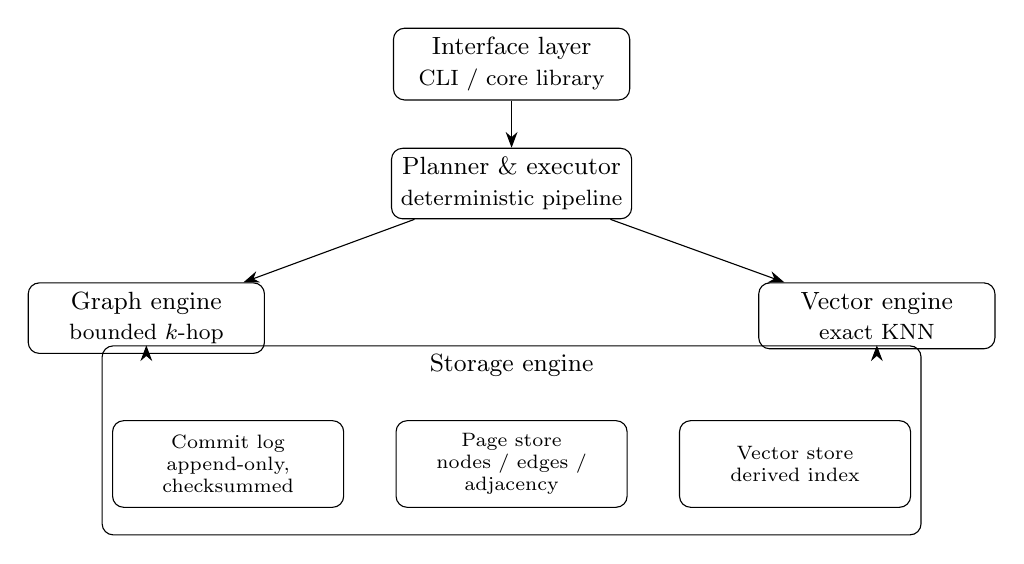
\begin{tikzpicture}[
  node distance=6mm and 10mm,
  box/.style={draw, rounded corners, align=center, minimum height=8mm, minimum width=30mm, font=\small},
  store/.style={draw, rounded corners, align=center, minimum height=11mm, text width=27mm, font=\scriptsize},
  >={Stealth[length=2mm]}
]
\node[box] (cli) {Interface layer\\\footnotesize CLI / core library};
\node[box, below=of cli] (plan) {Planner \& executor\\\footnotesize deterministic pipeline};
\node[box, below left=8mm and 16mm of plan] (graph) {Graph engine\\\footnotesize bounded $k$-hop};
\node[box, below right=8mm and 16mm of plan] (vec) {Vector engine\\\footnotesize exact KNN};
\node[draw, rounded corners, below=16mm of plan, minimum width=104mm, minimum height=24mm, font=\small] (storage) {};
\node[font=\small] at ([yshift=-2.5mm]storage.north) {Storage engine};
\node[store] (log) at ([xshift=-36mm,yshift=-3mm]storage.center) {Commit log\\append-only,\\checksummed};
\node[store] (base) at ([yshift=-3mm]storage.center) {Page store\\nodes / edges /\\adjacency};
\node[store] (vidx) at ([xshift=36mm,yshift=-3mm]storage.center) {Vector store\\derived index};
\draw[->] (cli) -- (plan);
\draw[->] (plan) -- (graph);
\draw[->] (plan) -- (vec);
\draw[->] (graph) -- (graph |- storage.north);
\draw[->] (vec) -- (vec |- storage.north);
\end{tikzpicture}
\caption{CheguersDB layered architecture. The commit log is the canonical
durability boundary; canonical graph and vector state is rebuilt from the log
(plus snapshots) on startup, and the vector index is treated as rebuildable
derived state.}
\label{fig:arch}
\end{figure}

\textbf{Interface layer.} A command-based CLI over the core library handles
ingestion and querying, validates payloads, and serialises results. The mutation
boundary is a typed command model.

\textbf{Planner and executor.} Execution is synchronous and single-process with a
deterministic operator order. Hybrid queries are composed as
\emph{vector\_search} $\rightarrow$ \emph{expand\_k\_hops} $\rightarrow$
\emph{rerank}, with bounded traversal depth and managed intermediate result sets.

\textbf{Vector engine.} The current release performs exact $k$-nearest-neighbour
retrieval over committed embeddings using cosine or $L_2$ similarity, with
deterministic tie-breaking by node identifier. ANN structures (HNSW, IVF,
quantisation) are deferred; embeddings are modelled as derived state that may be
rebuilt from canonical records.

\textbf{Graph engine.} Traversal uses forward adjacency with bounded depth
(1--3 hops) and deterministic output ordering.

\textbf{Storage engine.} The storage layer is the core of the contribution:
\begin{itemize}
  \item an \emph{append-only commit log} with a fixed record envelope, monotonic
  log indexes, per-record checksums, and tail-truncation / corruption handling,
  serving as the durable, ordered input to the state machine;
  \item a \emph{page-based object store} for nodes, edges, and adjacency
  segments, backed by file/page/header primitives, a disk-backed object heap, and
  simple free-space tracking;
  \item a \emph{snapshot} mechanism integrated with replay
  (snapshot $+$ log tail $\rightarrow$ state) to bound recovery time;
  \item \emph{canonical in-memory state} (nodes, edges, adjacency, vectors, and a
  primary-key index) reconstructed deterministically on startup.
\end{itemize}

\textbf{Key design decisions.} Canonical graph state is the source of truth;
the vector index is rebuildable derived state. The store uses page/segment
identifiers rather than raw physical pointers, easing recovery and on-disk format
evolution. Node and edge metadata are row-oriented. The release offers strong
local consistency. These choices follow lessons drawn selectively from
deterministic, replication-bounded designs~\cite{tigerbeetle} and from
graph-oriented storage layouts~\cite{kuzu,neo4j}.

\subsection{Software functionalities}
\label{sec:functionalities}

The implemented, user-facing capabilities are:
\begin{itemize}
  \item \textbf{Unified ingestion} of nodes, edges, and node-associated
  embeddings through a typed command model (\texttt{CreateNode},
  \texttt{CreateEdge}, \texttt{UpsertVector}, \texttt{DeleteNode},
  \texttt{DeleteEdge}, \texttt{DeleteVector}).
  \item \textbf{Durable writes with deterministic recovery}: log replay
  reconstructs the exact last committed prefix and recovers safely from truncated
  or corrupt log tails.
  \item \textbf{Vector top-$k$ retrieval} (exact, deterministic ordering).
  \item \textbf{Bounded $k$-hop traversal} over persisted adjacency.
  \item \textbf{End-to-end hybrid query}: top-$k$ $\rightarrow$ $k$-hop expansion
  $\rightarrow$ aggregation/rerank $\rightarrow$ final result set.
  \item \textbf{Snapshot and reopen}: state survives restart identically.
  \item \textbf{Reproducible benchmark harness}: seeded synthetic dataset
  generation, warmup, fixed measurement windows, multiple repetitions, and
  collection of p50/p95/p99 latency, throughput, and memory.
\end{itemize}

Correctness is guarded by an automated test suite covering codec round-trips,
replay correctness, recovery from truncated/corrupt tails, deterministic state
reconstruction, delete semantics, and end-to-end ``state survives restart''
behaviour.

%% ======================================================================
\section{Illustrative examples}
\label{sec:examples}

The following example demonstrates the full ingestion--recovery--query flow on a
small, seeded dataset. All commands are reproducible; outputs are deterministic
across repeated executions and across process restarts.

\textbf{1. Create a database and ingest a unified record.} A node may be ingested
together with its embedding and outgoing edges in a single operation:

\begin{lstlisting}
$ cheguers open ./demo.cdb
$ cheguers ingest --node '{"id":"123","label":"document",
    "properties":{"title":"example"}}' \
    --vector '[0.12, 0.98, ...]' \
    --edge '{"src":"123","dst":"456","type":"related"}'
\end{lstlisting}

\textbf{2. Recover and verify durability.} After reopening the database, committed
state is reconstructed by replaying the commit log (combined with the latest
snapshot). A node lookup returns the identical record ingested before restart,
demonstrating the recovery-first contract:

\begin{lstlisting}
$ cheguers reopen ./demo.cdb
$ cheguers get-node 123
node 123 (document) {title: "example"}  # identical pre/post restart
\end{lstlisting}

\textbf{3. Run a hybrid query.} A query embedding is resolved to its exact top-$k$
nearest nodes; each candidate is expanded by one graph hop; the union is reranked
by a deterministic rule and returned. Figure~\ref{fig:flow} shows the pipeline.

\begin{lstlisting}
$ cheguers hybrid --vector '[...]' --k 5 --depth 1
rank  node    score    via
1     123     0.981    candidate
2     456     0.944    expansion(123)
...   ...     ...      ...
\end{lstlisting}

\begin{figure}[!h]
\centering
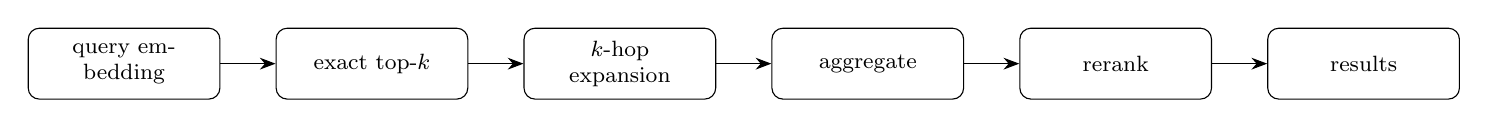
\begin{tikzpicture}[
  >={Stealth[length=2mm]},
  stage/.style={draw, rounded corners, align=center, minimum height=9mm, font=\footnotesize, text width=22mm},
  node distance=7mm
]
\node[stage] (q) {query embedding};
\node[stage, right=of q] (knn) {exact top-$k$};
\node[stage, right=of knn] (exp) {$k$-hop\\expansion};
\node[stage, right=of exp] (agg) {aggregate};
\node[stage, right=of agg] (rr) {rerank};
\node[stage, right=of rr] (out) {results};
\draw[->] (q) -- (knn);
\draw[->] (knn) -- (exp);
\draw[->] (exp) -- (agg);
\draw[->] (agg) -- (rr);
\draw[->] (rr) -- (out);
\end{tikzpicture}
\caption{Deterministic hybrid query pipeline: vector top-$k$ retrieval, bounded
graph expansion of each candidate, aggregation, and reranking.}
\label{fig:flow}
\end{figure}

\textbf{Measured behaviour.} On a seeded synthetic dataset of
\PLACEHOLDER{N} nodes and \PLACEHOLDER{M} edges with embedding dimension
\PLACEHOLDER{d}, under the harness protocol (warmup, fixed
\PLACEHOLDER{60}\,s window, \PLACEHOLDER{R} repetitions, fixed seed), CheguersDB
achieves p50/p95 latencies of \PLACEHOLDER{x/y}\,ms for vector top-$k$,
\PLACEHOLDER{x/y}\,ms for $k$-hop traversal, and \PLACEHOLDER{x/y}\,ms for the
hybrid query, sustaining \PLACEHOLDER{Q}\,QPS at a resident memory footprint of
\PLACEHOLDER{Z}. Full results, including p99 and scaling curves, are reported in
the repository.

%% --- AUTHOR: insert benchmark results figure here (Figure 3) ---
% \begin{figure}[!h]\centering
%   \includegraphics[width=.8\linewidth]{fig_results.pdf}
%   \caption{p50/p95/p99 latency for vector, traversal, and hybrid queries.}
%   \label{fig:results}
% \end{figure}

%% ======================================================================
\section{Impact}
\label{sec:impact}

\textbf{New research questions enabled.} By co-locating graph topology and
embeddings in a single engine with a deterministic execution path, CheguersDB
makes it possible to study the cost structure of hybrid retrieval in isolation:
in particular, the incremental latency of the graph-expansion phase \emph{after}
ANN candidate selection, and how that cost scales with candidate-set size, fan-out,
and embedding dimensionality. These interaction effects are difficult to attribute
cleanly in composed stacks, where two independent systems and a network boundary
confound measurement. The bundled, seeded harness allows others to reproduce and
extend these experiments.

\textbf{Improving existing research questions.} For HybridRAG research and for
agent / copilot / contextual-search builders, the engine removes the two-system
orchestration burden and provides a crash-recoverable, reproducible retrieval
substrate. Because canonical state is defined by a replayable log rather than by
two separately-updated indexes, experimental results are reproducible across runs
and restarts --- a property that strengthens the empirical validity of HybridRAG
evaluations.

\textbf{Methodological contribution.} The artifact demonstrates that a
correctness-first foundation (append-only log plus deterministic replay) is a
viable base for unified graph--vector serving, and it provides an open benchmark
methodology for \emph{hybrid} workloads that combines kernels (isolated ANN,
isolated traversal) with end-to-end compositions, addressing the absence of
standard benchmarks for this class of system.

\textbf{Roadmap and potential impact.} The architecture is designed to extend
beyond the single node. Planned directions, layered around the deterministic
apply boundary, include per-shard-group replication informed by
deterministic distributed designs~\cite{tigerbeetle}, HNSW~\cite{hnsw} introduced
as a derived index attached to a snapshot watermark, locality-aware sharding by
source-node identifier, and access-control-aware retrieval. These are presented
as future work; the current release establishes the foundation on which they
build.

%% --- AUTHOR: insert baseline-comparison figure here (Figure 4), once measured ---
% Compare CheguersDB against a composed stack (Neo4j + Qdrant) and/or an
% integrated engine (HelixDB) on the SAME hybrid workload.

%% ======================================================================
\section{Conclusions}
\label{sec:conclusions}

CheguersDB is an open-source Rust storage engine that unifies graph and vector
data within one deterministic execution path for HybridRAG retrieval. This
release delivers and validates a single-node, recovery-first serving kernel: an
append-only commit log with deterministic crash-replay, a page-based graph store,
exact $k$-nearest-neighbour retrieval, bounded $k$-hop traversal, an end-to-end
hybrid query pipeline, and a reproducible benchmark harness, all backed by an
automated test suite. By making canonical state replayable and hybrid retrieval
reproducible, the engine offers a crash-recoverable alternative to composed
graph-plus-vector stacks and a clean instrument for studying the cost of hybrid
retrieval. Distributed execution, approximate indexing, and access control are
deferred by design; the durable, deterministic kernel described here is the
foundation on which those extensions will be built.

\section*{Acknowledgements}

The authors thank \PLACEHOLDER{advisors / Inteli / contributors} for their
support during the development of CheguersDB.

%% ---------------------------------------------------------------------------
%% Declaration of generative AI use (include ONLY if applicable; otherwise delete)
% \section*{Declaration of generative AI and AI-assisted technologies in the manuscript preparation process}
% During the preparation of this work the author(s) used [TOOL] in order to [REASON].
% After using this tool, the author(s) reviewed and edited the content as needed and
% take(s) full responsibility for the content of the published article.

\begin{thebibliography}{00}

\bibitem{peng2024graphrag} Peng B, et al. Graph retrieval-augmented generation: a survey. arXiv:2408.08921; 2024. \url{https://arxiv.org/abs/2408.08921}.

\bibitem{hybridrag2025} HybridRAG: integrating knowledge graphs and vector retrieval for efficient information extraction. Proc. ACL; 2025.

\bibitem{helixdb} HelixDB. Hybrid graph--vector database [software]. \url{https://www.helix-db.com} [accessed \PLACEHOLDER{date}].

\bibitem{neo4j} Neo4j Inc. Neo4j graph database [software]. \url{https://neo4j.com} [accessed \PLACEHOLDER{date}].

\bibitem{qdrant} Qdrant. Vector database [software]. \url{https://qdrant.tech} [accessed \PLACEHOLDER{date}].

\bibitem{milvus} Milvus: a cloud-native vector database [software]. \url{https://milvus.io} [accessed \PLACEHOLDER{date}].

\bibitem{weaviate} Weaviate: open-source vector database [software]. \url{https://weaviate.io} [accessed \PLACEHOLDER{date}].

\bibitem{tigerbeetle} TigerBeetle: a distributed financial accounting database [software]. \url{https://tigerbeetle.com} [accessed \PLACEHOLDER{date}].

\bibitem{kuzu} K\`uzu: an embedded property graph database [software]. \url{https://github.com/kuzudb/kuzu} [accessed \PLACEHOLDER{date}].

\bibitem{janusgraph} JanusGraph: distributed graph database [software]. \url{https://janusgraph.org} [accessed \PLACEHOLDER{date}].

\bibitem{hnsw} Malkov YA, Yashunin DA. Efficient and robust approximate nearest neighbor search using hierarchical navigable small world graphs. IEEE Trans Pattern Anal Mach Intell 2020;42(4):824-36. \url{https://doi.org/10.1109/TPAMI.2018.2889473}.

\end{thebibliography}

\end{document}
